\documentclass{ctexbeamer}

\usepackage{bm}
\usepackage{graphicx}
\usepackage{color}

\usetheme[colorblocks, sidebar]{Verona}
\usefonttheme[onlymath]{serif}




\title{合并同类项}
\subtitle{Unite Like Terms}
%\author{授课人:邱鹏}
%\institute{黄桥镇中学}
\date{\today}
\logo{
\includegraphics[height=1.2cm]{assets/Pngtree owl double exposure.png}}

\AtBeginSection[]
{
	\begin{frame}{目录}
		\tableofcontents[currentsection]
	\end{frame}
}

\usepackage{fontspec}
\setromanfont{EB Garamond}
\usefonttheme{serif}

\begin{document}


\begin{frame}
	\titlepage
\end{frame}

\begin{frame}{新课导入}
	
	\begin{block}{}
	我们知道 $ 2 + 4 = 6 $, 那么 $ 2x + 4x $ 是否等于 $ 6x $ 呢?
	\end{block}
	
	\begin{figure}
		
\includegraphics[width = 2.4cm]{assets/Pngtree student thinking.png}
	\end{figure}

	\pause
	\begin{block}{$2$个$x$ 加上  $4$ 个 $x$, 一共  $6$ 个  $x$ :}
		 
		\[
			\bm{2x + 4x = (2 + 4)x = 6x}
		\]
	\end{block}

	\begin{columns}
		\column{0.49\textwidth}
			\begin{alertblock}{乘法分配律}
				$$ \bm{ac + bc = (a + b)c} $$
			\end{alertblock}
		\column{0.49\textwidth}
			\begin{figure}
				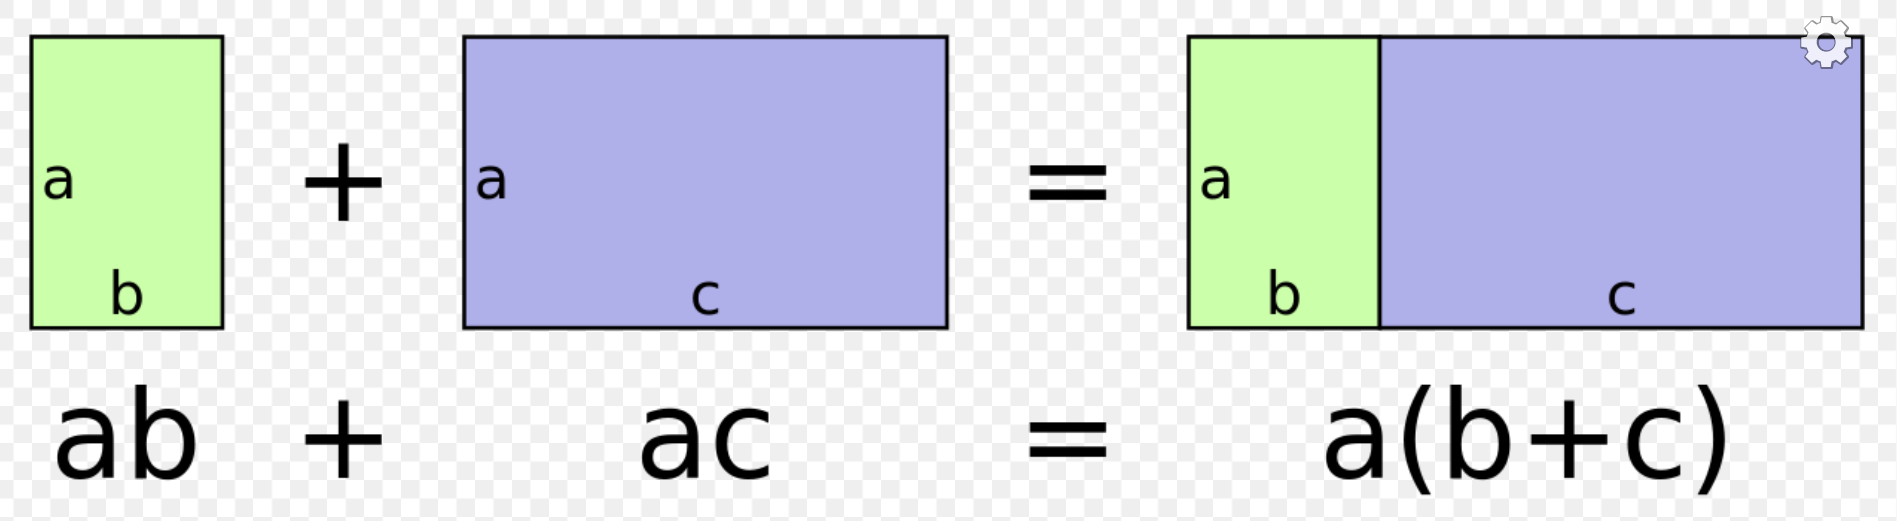
\includegraphics[width = 0.75\textwidth]{assets/dist law.png}
			\end{figure}
	\end{columns}
	

\end{frame}

\begin{frame}{情景导入}
	\begin{columns}
		\column{0.4\textwidth}
			\begin{figure}
				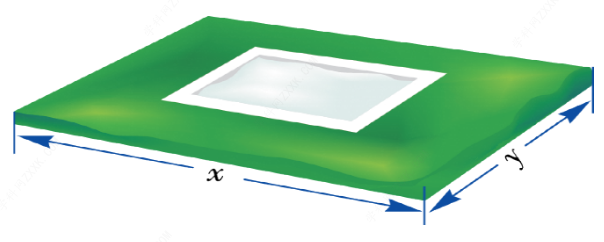
\includegraphics[width = 0.9\textwidth]{assets/meadow.png}
			\end{figure}
		\column{0.58\textwidth}
			\begin{block}{}
			如图,在一块长为 $x$, 宽为 $y$ 的草地中间,挖了一个面积为 $ \frac{1}{3}
			xy $ 的水池后,剩余草地的面积是多少?
			\end{block}
	\end{columns}

	\vspace{0.5cm}
	\begin{enumerate}
		\item<2-> {列出求剩余草地面积代数式}  $$ \bm{xy - \frac{1}{3}xy} $$
		\item<3-> {化简,合并同类项($1$份$xy$减去$\frac{1}{3}$份$xy$)}  
			$$ \bm{xy - \frac{1}{3}xy = (1-\frac{1}{3})xy = \frac{2}{3}xy} $$
			\begin{alertblock}{乘法分配律}
				$$ \bm{ac + bc = (a + b)c} $$
			\end{alertblock}
	\end{enumerate}
\end{frame}

\section{一:同类项的定义}
	\begin{frame}{WHAT - 什么是同类项?}
		\begin{columns}[t]
			\column{0.49\textwidth}
			\begin{alertblock}{概念}
				含有的字母相同,并且相同字母的指数也分别相同的项,
				称它们为\\ \alert{同类项}(Like Term)。
			\end{alertblock}
			
			\column{0.48\textwidth}
			\begin{examples}
				$ -ab^2 $ 和 $ 5ab^2 $ 都含有字母 $ a $, $ b $, 
				且\\ $ a $ 的次数都是 $ 1 $, $ b $ 的次数都是 $ 2 $, 
				所以二者是同类项。
			\end{examples}
		\end{columns}
	\end{frame}

	\begin{frame}{同类项}
		\begin{block}{注意}
			\begin{itemize}
				\item 两个相同:字母相同,同一字母的次数相同。
				\item 两个无关:与系数无关,与字母顺序无关。
				\item \alert{所有的常数项都是同类项}。
			\end{itemize}
		\end{block}
			
		\vspace{1cm}
		\begin{columns}
			\column{0.49\textwidth}
			$xy - \frac{1}{3}xy$
				\begin{flushleft}
				\begin{tabular}{|rrr|}
					\hline
					项   &    系数    & 字母部分 \\ 
					\hline
					$xy$ &    $1$    & $xy$  \\  
					\hline
					$-\frac{1}{3}xy$ & $-\frac{1}{3}$ & $xy$ \\
					\hline
				\end{tabular}
				\end{flushleft}

			\column{0.49\textwidth}
			$x^2y + 3x + 1 -4x -\frac{4}{3}yx^2 - 5$
			\begin{flushleft}
				\begin{tabular}{|rrr|}
					\hline
					项   &    系数    & 字母部分 \\ 
					\hline
					$x^2y$ &    $1$    & $x^2y$  \\  
					\hline
					$-\frac{4}{3}yx^2$ & $-\frac{4}{3}$ & $yx^2$ \\
					\hline
				\end{tabular}
			\end{flushleft}
		\end{columns}
	\end{frame}

	\begin{frame}{练习}
		\only<1>{
			\begin{figure}
				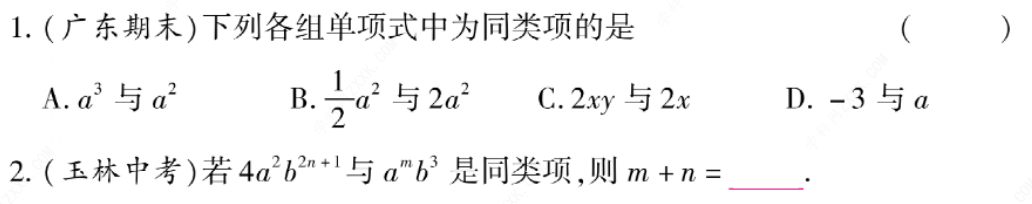
\includegraphics[width=.9\textwidth]{assets/like term.png}
			\end{figure}
		}

		\only<2->{
			\begin{figure}
				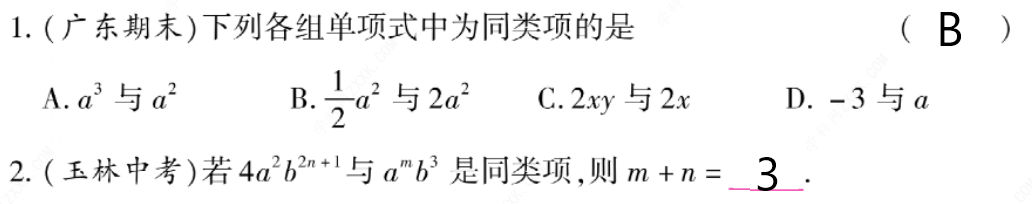
\includegraphics[width=.9\textwidth]{assets/like term2.png}
			\end{figure}
		}
	\end{frame}
	
\section{二:合并同类项}
	\begin{frame}{合并同类项}
		\begin{block}{}
			把多项式中的同类项合并成一项,叫做 \alert{合并同类项(Unite Like Terms)}
		\end{block}
	\end{frame}

	\begin{frame}{HOW - 如何合并同类项}

		\begin{block}{}
			\[
				\bm{2x + 4x = (2 + 4)x =6x}
			\]
		\end{block}
		\begin{block}{}
			$$ \bm{xy - \frac{1}{3}xy = (1-\frac{1}{3})xy = \frac{2}{3}xy} $$
		\end{block}

		\begin{alertblock}{}
			$$ \bm{ac + bc = (a + b)c} $$
		\end{alertblock}

		\pause
		\begin{block}{}
			合并同类项时,只要把它们的系数相加,字母和字母的指数不变,\\
			即“\alert{一相加,两不变}”。
			一相加是把系数相加,两不变就是字母不变,字母的指数不变。
		\end{block}
	\end{frame}

	\begin{frame}{合并同类项的步骤}
		\begin{itemize}
			\item 找,找出多项式中的同类项
			\item 移,利用加法交换律和结合律,把多项式中的同类项交换位置结合在一起,没有同类项的照抄
			\item 合,将同类项的系数相加,字母和字母的指数不变
		\end{itemize}

		\begin{example}{合并同类项}
			$4x^2y-8xy^2+7-4x^2y+10xy^2-4$\\
			\pause
			\only<2>{
				\textbf{解\hspace{0.2cm}原式}
				$ = 4x^2y-4x^2y-8xy^2+10xy^2+7-4$\\
				\hspace{1.48cm}$ = (4x^2y-4x^2y)+(-8xy^2+10xy^2)+(7-4)$\\
				\hspace{1.48cm}$ = (4-4)x^2y+ (-8+10)xy^2+(7-4)$ \\
				\hspace{1.48cm}$ = 2xy^2+3 $
			}
		\end{example}
	\end{frame}

	\begin{frame}{合并同类项时,要注意}
		\begin{block}{}
			\begin{itemize}
				\item<1-> 移动位置时要连同它前面的符号一起移动。
				%\item<1-> 把减法化成加法,减去一个数等于加上这个数的相反数。
				\item<2-> 系数相加时,要注意符号。
			\end{itemize}
		\end{block}

		\begin{example}{合并同类项}
			$4x^2y \bm{-8xy^2} +7-4x^2y+10xy^2-4$\\

				\textbf{解\hspace{0.2cm}原式}
				$ = 4x^2y-4x^2y\bm{-8xy^2}+10xy^2+7-4$\\
				\hspace{1.48cm}$ = (4x^2y-4x^2y)+(\bm{-8xy^2}+10xy^2)+(7-4)$\\
				\hspace{1.48cm}$ = (4-4)x^2y+ (\bm{-8}+10)xy^2+(7-4)$ \\
				\hspace{1.48cm}$ = 2xy^2+3 $
		\end{example}
	\end{frame}

	\begin{frame}{合并同类项 - 练习}
		\only<1>{
			\begin{figure}
				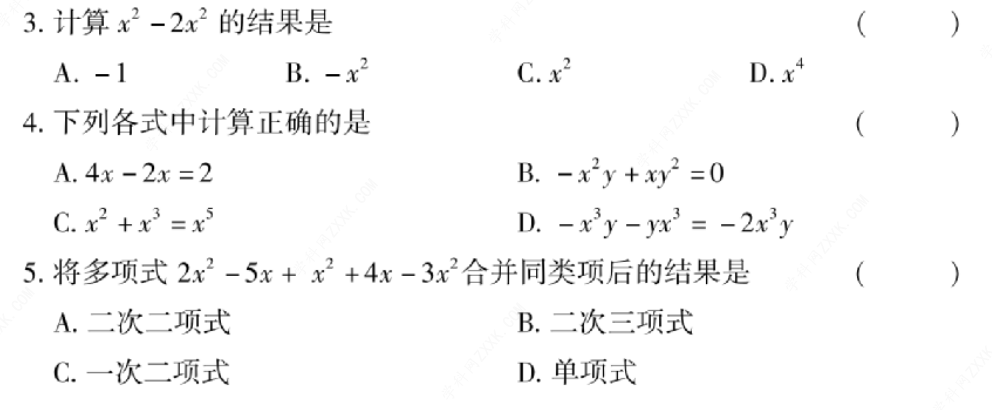
\includegraphics[width=.9\textwidth]{assets/like term3.png}
			\end{figure}
		}

		\only<2->{
			\begin{figure}
				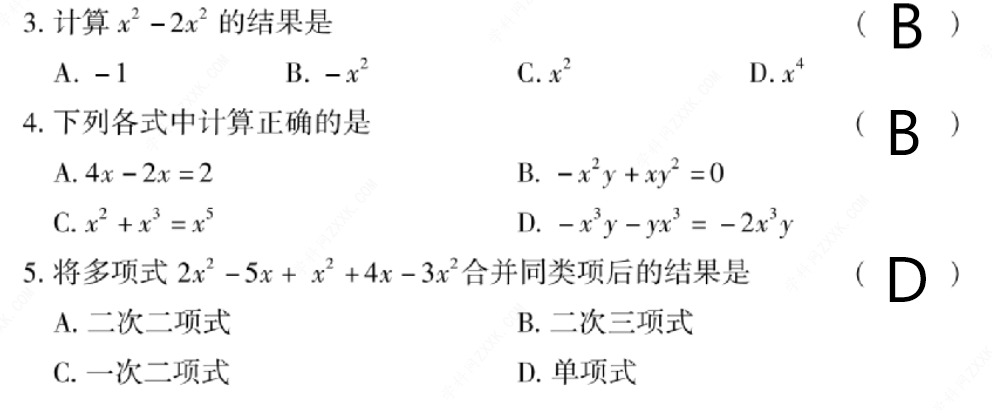
\includegraphics[width=.9\textwidth]{assets/like term4.png}
			\end{figure}
		}
	\end{frame}

\end{document}